\documentclass[tikz,border=7pt]{standalone}

\usepackage{iftex}
\ifPDFTeX
  \PackageError{matrix-figure}{This figure requires XeTeX or Tectonic}{Compile with xelatex or tectonic.}
\fi
\usepackage{fontspec}
\usepackage{xeCJK}
\usepackage{amsmath}
\usepackage{unicode-math}
\usepackage{xcolor}
\usepackage{tikz}
\usetikzlibrary{arrows.meta,positioning}

\providecommand{\FigureUseLocalFonts}{0}
\ifnum\FigureUseLocalFonts=1
  \setmainfont{NotoSansCJKtc-Regular.otf}[Path=\FigureSansFontPath]
  \setsansfont{NotoSansCJKtc-Regular.otf}[Path=\FigureSansFontPath,BoldFont=NotoSansCJKtc-Bold.otf]
  \setCJKmainfont{NotoSansCJKtc-Regular.otf}[Path=\FigureSansFontPath]
  \setCJKsansfont{NotoSansCJKtc-Regular.otf}[Path=\FigureSansFontPath,BoldFont=NotoSansCJKtc-Bold.otf]
  \setmathfont{STIXTwoMath.otf}[Path=\FigureMathFontPath]
\else
  \setmainfont{Noto Sans CJK TC}
  \setsansfont{Noto Sans CJK TC}
  \setCJKmainfont{Noto Sans CJK TC}
  \setCJKsansfont{Noto Sans CJK TC}
  \setmathfont{STIX Two Math}
\fi

\definecolor{FigureInk}{HTML}{253142}
\definecolor{StageOne}{gray}{0.94}
\definecolor{StageTwo}{gray}{0.90}
\definecolor{StageThree}{gray}{0.84}

\newcommand{\FigureAugMatrix}[1]{%
  \renewcommand{\arraystretch}{1.25}%
  \left[\begin{array}{ccc|c}#1\end{array}\right]%
}

\begin{document}
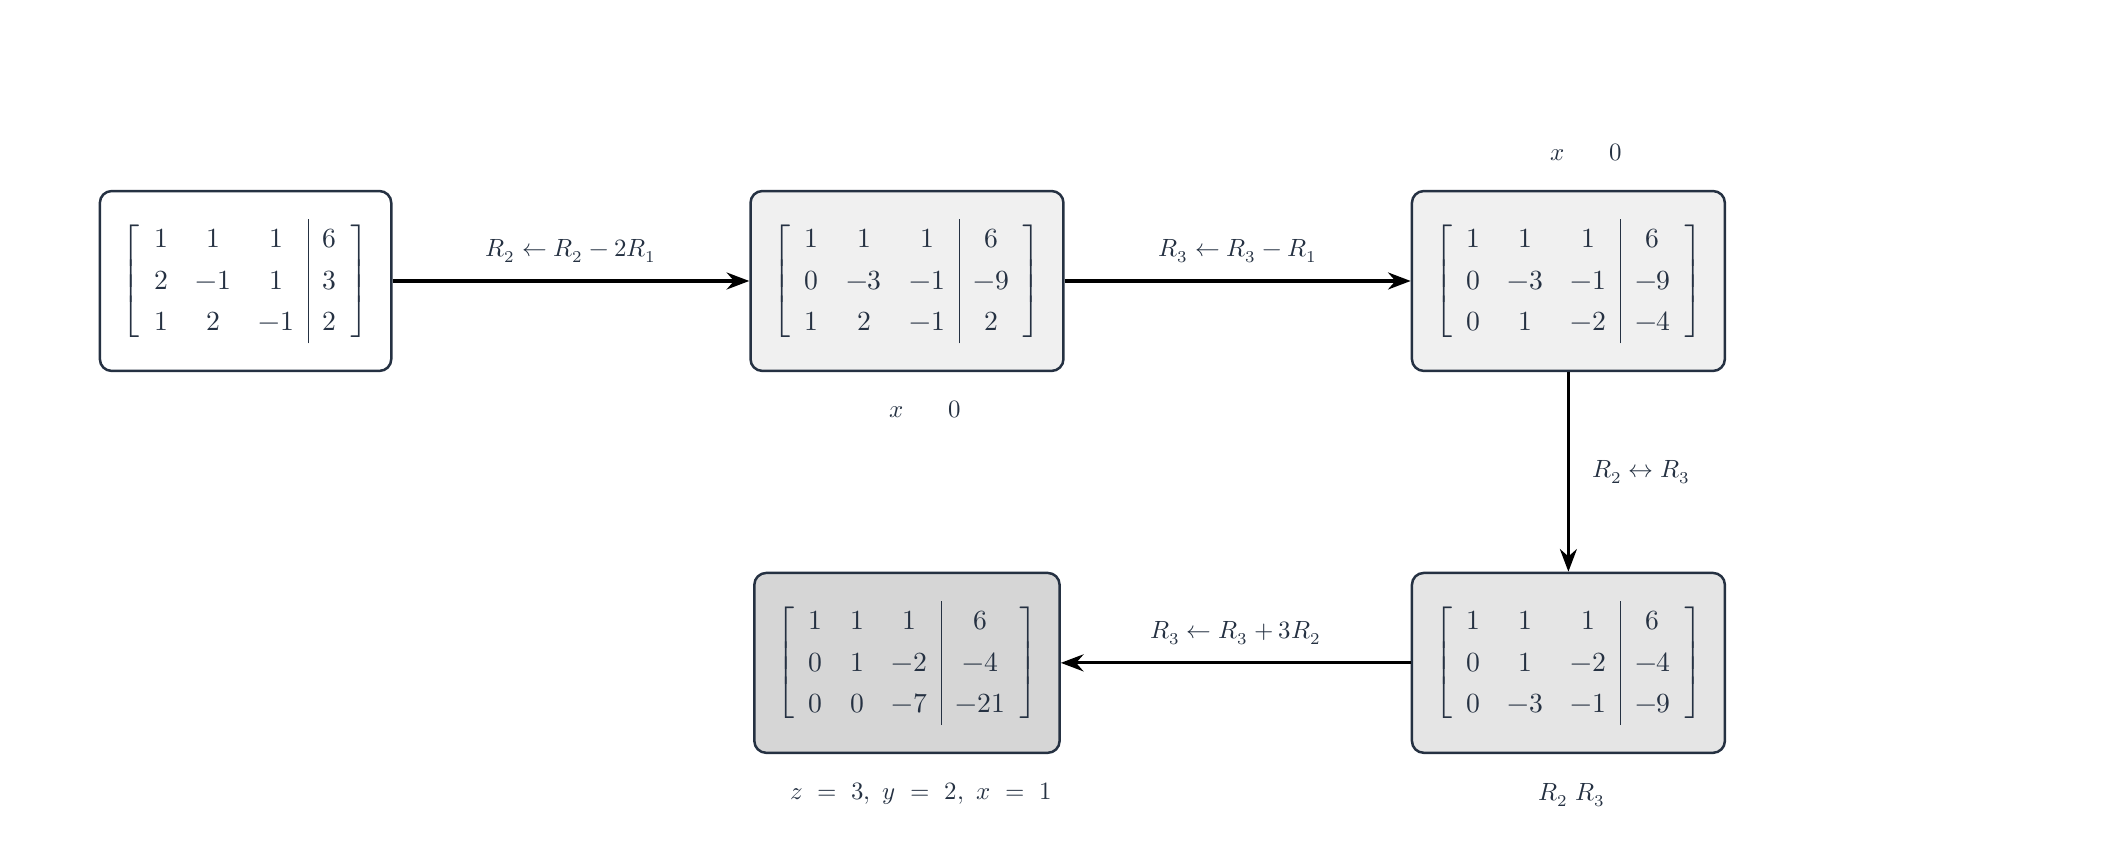
\begin{tikzpicture}[
  font=\sffamily,
  text=FigureInk,
  >={Stealth[length=4mm,width=2.7mm]},
  stage/.style={draw=FigureInk,line width=0.9pt,rounded corners=1.5mm,inner xsep=8pt,inner ysep=10pt},
  operation/.style={align=center,font=\small,fill=white,inner sep=2pt},
  caption/.style={align=center,font=\bfseries\small,text width=5.1cm},
]
  \node[font=\bfseries\Large,align=center,text width=26cm] at (13.05,9.40)
    {高斯消去的逐步列運算};

  \node[stage,fill=white] (m0) at (2.70,6.30) {$
    \FigureAugMatrix{1&1&1&6\\2&-1&1&3\\1&2&-1&2}
  $};
  \node[stage,fill=StageOne] (m1) at (11.10,6.30) {$
    \FigureAugMatrix{1&1&1&6\\0&-3&-1&-9\\1&2&-1&2}
  $};
  \node[stage,fill=StageOne] (m2) at (19.50,6.30) {$
    \FigureAugMatrix{1&1&1&6\\0&-3&-1&-9\\0&1&-2&-4}
  $};
  \node[stage,fill=StageTwo] (m3) at (19.50,1.45) {$
    \FigureAugMatrix{1&1&1&6\\0&1&-2&-4\\0&-3&-1&-9}
  $};
  \node[stage,fill=StageThree] (m4) at (11.10,1.45) {$
    \FigureAugMatrix{1&1&1&6\\0&1&-2&-4\\0&0&-7&-21}
  $};

  \draw[-{Stealth},line width=1.15pt] (m0.east) --
    node[operation,above=4pt] {$R_2\leftarrow R_2-2R_1$}
    (m1.west);
  \draw[-{Stealth},line width=1.15pt] (m1.east) --
    node[operation,above=4pt] {$R_3\leftarrow R_3-R_1$}
    (m2.west);
  \draw[-{Stealth},line width=1.15pt] (m2.south) --
    node[operation,right=6pt] {$R_2\leftrightarrow R_3$}
    (m3.north);
  \draw[-{Stealth},line width=1.15pt] (m3.west) --
    node[operation,above=4pt] {$R_3\leftarrow R_3+3R_2$}
    (m4.east);

  \node[caption,below=7pt of m0] {原增廣矩陣};
  \node[caption,below=7pt of m1] {第二列的 $x$ 係數消成 $0$};
  \node[caption,above=7pt of m2] {第三列的 $x$ 係數消成 $0$};
  \node[caption,below=7pt of m3] {交換 $R_2$、$R_3$ 後};
  \node[caption,below=7pt of m4] {階梯形：$z=3,\ y=2,\ x=1$};
\end{tikzpicture}
\end{document}
